% ============================================================================
% CSCE 763: Digital Image Processing - Midterm Exam (Fall 2022)
% ============================================================================

\documentclass[12pt]{article}

% ============================================================================
% PACKAGE IMPORTS
% ============================================================================
\usepackage{amsmath}
\usepackage{graphicx}
\usepackage{amssymb}
\usepackage{tikz}
\usepackage[margin=1in]{geometry}
\usepackage{setspace}
\usepackage{xcolor}
\usepackage{enumitem}
\usepackage{tcolorbox}
\usepackage{fancyhdr}
\usepackage{booktabs}
\usepackage{array}
\usepackage{colortbl}
\usepackage{float}

% ============================================================================
% HEADER AND FOOTER SETUP
% ============================================================================
\pagestyle{fancy}
\setlength{\headheight}{14.5pt}
\fancyhf{}

\fancyhead[L]{Midterm Fa22}
\fancyhead[R]{CSCE 763: Digital Image Processing}

\renewcommand{\headrulewidth}{0pt}

% ============================================================================
% TIKZ LIBRARIES
% ============================================================================
\usetikzlibrary{shapes.geometric, arrows.meta, positioning, patterns, calc}

% --- USC Brand Colors ---
\definecolor{USC_Garnet}{HTML}{73000A}
\definecolor{USC_Sandstorm}{HTML}{FFF2E3}
\definecolor{USC_Black90}{HTML}{363636}
\definecolor{USC_Black70}{HTML}{5C5C5C}
\definecolor{USC_Black50}{HTML}{A2A2A2}
\definecolor{USC_Black10}{HTML}{ECECEC}
\definecolor{USC_Honeycomb}{HTML}{65780B}
\definecolor{USC_Atlantic}{HTML}{466A9F}
\definecolor{USC_Congaree}{HTML}{1F414D}
\definecolor{USC_Rose}{HTML}{CC2E40}

% ============================================================================
% CUSTOM COLORED BOXES
% ============================================================================
\newtcolorbox{stepbox}[1][Step]{
  colback=white,
  colframe=USC_Garnet,
  fonttitle=\bfseries,
  title=#1,
  sharp corners,
  colbacktitle=USC_Garnet,
  coltitle=white,
}

\newtcolorbox{resultsbox}{
  colback=white,
  colframe=USC_Honeycomb,
  fonttitle=\bfseries,
  title=Results,
  sharp corners,
  colbacktitle=USC_Honeycomb,
  coltitle=white,
}

% ============================================================================
% CUSTOM QUESTION COMMANDS
% ============================================================================
\newcommand{\problem}[1]{%
  \vspace{0.5cm}
  {\noindent\normalsize \textbf{#1}}
  \vspace{0.3cm}
}

% ============================================================================
% DOCUMENT INFORMATION
% ============================================================================

\title{\textbf{Midterm Exam}}
\author{}
\date{}

% ============================================================================
% BEGIN DOCUMENT
% ============================================================================

\begin{document}

\thispagestyle{fancy}
\setlength{\parindent}{0pt}

\setlist[enumerate,1]{label=\alph*)}
\setlist[enumerate,2]{label=(\roman*)}

% ============================================================================
% PROBLEM 1
% ============================================================================

\problem{Problem 1a) (15 points)}

Given the image region as shown in Figure 1 and $V = \{1\}$, what is the shortest m-path between $p$
(the pixel at the upper-left corner) and $q$ (the pixel at the bottom-right corner)? Give the length of
the path if the path exists.

\begin{center}
$\begin{array}{ccccc}
1 & 0 & 1 & 1 & 0 \\
0 & 1 & 0 & 1 & 0 \\
0 & 0 & 1 & 1 & 0 \\
1 & 1 & 0 & 1 & 0 \\
0 & 1 & 1 & 1 & 1
\end{array}$
\end{center}

\vspace{0.5cm}

\begin{stepbox}[Step 1: Identify pixels in $V = \{1\}$]

\begin{center}
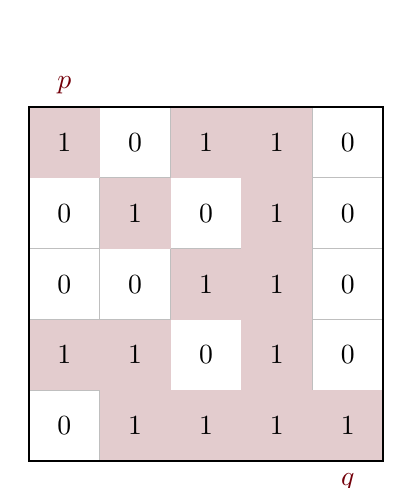
\begin{tikzpicture}[scale=0.9]
    % Draw grid
    \foreach \x in {0,1,2,3,4,5} {
        \draw[gray!50] (\x,0) -- (\x,5);
        \draw[gray!50] (0,\x) -- (5,\x);
    }

    % Highlight V={1} pixels (row 0 is at top, so y = 4-row)
    % Row 0: (0,0)=1, (0,2)=1, (0,3)=1
    \fill[USC_Garnet!20] (0,4) rectangle (1,5);
    \fill[USC_Garnet!20] (2,4) rectangle (3,5);
    \fill[USC_Garnet!20] (3,4) rectangle (4,5);
    % Row 1: (1,1)=1, (1,3)=1
    \fill[USC_Garnet!20] (1,3) rectangle (2,4);
    \fill[USC_Garnet!20] (3,3) rectangle (4,4);
    % Row 2: (2,2)=1, (2,3)=1
    \fill[USC_Garnet!20] (2,2) rectangle (3,3);
    \fill[USC_Garnet!20] (3,2) rectangle (4,3);
    % Row 3: (3,0)=1, (3,1)=1, (3,3)=1
    \fill[USC_Garnet!20] (0,1) rectangle (1,2);
    \fill[USC_Garnet!20] (1,1) rectangle (2,2);
    \fill[USC_Garnet!20] (3,1) rectangle (4,2);
    % Row 4: (4,1)=1, (4,2)=1, (4,3)=1, (4,4)=1
    \fill[USC_Garnet!20] (1,0) rectangle (2,1);
    \fill[USC_Garnet!20] (2,0) rectangle (3,1);
    \fill[USC_Garnet!20] (3,0) rectangle (4,1);
    \fill[USC_Garnet!20] (4,0) rectangle (5,1);

    % Fill in values
    \node at (0.5,4.5) {1}; \node at (1.5,4.5) {0}; \node at (2.5,4.5) {1}; \node at (3.5,4.5) {1}; \node at (4.5,4.5) {0};
    \node at (0.5,3.5) {0}; \node at (1.5,3.5) {1}; \node at (2.5,3.5) {0}; \node at (3.5,3.5) {1}; \node at (4.5,3.5) {0};
    \node at (0.5,2.5) {0}; \node at (1.5,2.5) {0}; \node at (2.5,2.5) {1}; \node at (3.5,2.5) {1}; \node at (4.5,2.5) {0};
    \node at (0.5,1.5) {1}; \node at (1.5,1.5) {1}; \node at (2.5,1.5) {0}; \node at (3.5,1.5) {1}; \node at (4.5,1.5) {0};
    \node at (0.5,0.5) {0}; \node at (1.5,0.5) {1}; \node at (2.5,0.5) {1}; \node at (3.5,0.5) {1}; \node at (4.5,0.5) {1};

    % Label p and q
    \node[USC_Garnet, font=\bfseries] at (0.5,5.3) {$p$};
    \node[USC_Garnet, font=\bfseries] at (4.5,-0.3) {$q$};

    % Draw outer border
    \draw[thick] (0,0) rectangle (5,5);
\end{tikzpicture}
\end{center}

All pixels with value 1 are highlighted. These are the only candidates for the m-path since $V = \{1\}$.

\end{stepbox}

\begin{stepbox}[Step 2: Apply m-adjacency rules]

Two pixels with values in $V$ are \textbf{m-adjacent} if:
\begin{enumerate}[leftmargin=2em, itemsep=0pt]
    \item They are 4-adjacent (share an edge), OR
    \item They are diagonally adjacent AND their shared 4-neighbors contain no pixels with values in $V$.
\end{enumerate}

The second condition prevents diagonal shortcuts when a 4-connected bridge exists, eliminating path ambiguity.

\end{stepbox}

\begin{stepbox}[Step 3: Trace the shortest m-path]

\begin{center}
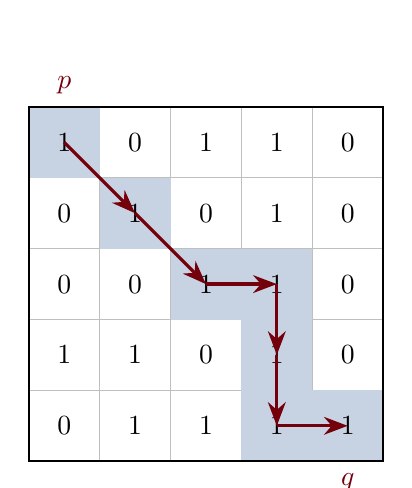
\begin{tikzpicture}[scale=0.9]
    % Draw grid
    \foreach \x in {0,1,2,3,4,5} {
        \draw[gray!50] (\x,0) -- (\x,5);
        \draw[gray!50] (0,\x) -- (5,\x);
    }

    % Highlight path pixels
    \fill[USC_Atlantic!30] (0,4) rectangle (1,5);   % (0,0)
    \fill[USC_Atlantic!30] (1,3) rectangle (2,4);   % (1,1)
    \fill[USC_Atlantic!30] (2,2) rectangle (3,3);   % (2,2)
    \fill[USC_Atlantic!30] (3,2) rectangle (4,3);   % (2,3)
    \fill[USC_Atlantic!30] (3,1) rectangle (4,2);   % (3,3)
    \fill[USC_Atlantic!30] (3,0) rectangle (4,1);   % (4,3)
    \fill[USC_Atlantic!30] (4,0) rectangle (5,1);   % (4,4)

    % Fill in values
    \node at (0.5,4.5) {1}; \node at (1.5,4.5) {0}; \node at (2.5,4.5) {1}; \node at (3.5,4.5) {1}; \node at (4.5,4.5) {0};
    \node at (0.5,3.5) {0}; \node at (1.5,3.5) {1}; \node at (2.5,3.5) {0}; \node at (3.5,3.5) {1}; \node at (4.5,3.5) {0};
    \node at (0.5,2.5) {0}; \node at (1.5,2.5) {0}; \node at (2.5,2.5) {1}; \node at (3.5,2.5) {1}; \node at (4.5,2.5) {0};
    \node at (0.5,1.5) {1}; \node at (1.5,1.5) {1}; \node at (2.5,1.5) {0}; \node at (3.5,1.5) {1}; \node at (4.5,1.5) {0};
    \node at (0.5,0.5) {0}; \node at (1.5,0.5) {1}; \node at (2.5,0.5) {1}; \node at (3.5,0.5) {1}; \node at (4.5,0.5) {1};

    % Draw arrows for m-path
    \draw[-{Stealth[length=3mm]}, USC_Garnet, very thick] (0.5,4.5) -- (1.5,3.5);  % (0,0) -> (1,1) diagonal
    \draw[-{Stealth[length=3mm]}, USC_Garnet, very thick] (1.5,3.5) -- (2.5,2.5);  % (1,1) -> (2,2) diagonal
    \draw[-{Stealth[length=3mm]}, USC_Garnet, very thick] (2.5,2.5) -- (3.5,2.5);  % (2,2) -> (2,3) horizontal
    \draw[-{Stealth[length=3mm]}, USC_Garnet, very thick] (3.5,2.5) -- (3.5,1.5);  % (2,3) -> (3,3) vertical
    \draw[-{Stealth[length=3mm]}, USC_Garnet, very thick] (3.5,1.5) -- (3.5,0.5);  % (3,3) -> (4,3) vertical
    \draw[-{Stealth[length=3mm]}, USC_Garnet, very thick] (3.5,0.5) -- (4.5,0.5);  % (4,3) -> (4,4) horizontal

    % Label p and q
    \node[USC_Garnet, font=\bfseries] at (0.5,5.3) {$p$};
    \node[USC_Garnet, font=\bfseries] at (4.5,-0.3) {$q$};

    % Draw outer border
    \draw[thick] (0,0) rectangle (5,5);
\end{tikzpicture}
\end{center}

\textbf{Path:} $(0,0) \to (1,1) \to (2,2) \to (2,3) \to (3,3) \to (4,3) \to (4,4)$

\vspace{0.2cm}

\textbf{Diagonal move justifications:}
\begin{itemize}[leftmargin=2em, itemsep=0pt]
    \item $(0,0) \to (1,1)$: Shared 4-neighbors are $(0,1)=0$ and $(1,0)=0$. Neither is in $V$, so m-adjacent.
    \item $(1,1) \to (2,2)$: Shared 4-neighbors are $(1,2)=0$ and $(2,1)=0$. Neither is in $V$, so m-adjacent.
\end{itemize}

\end{stepbox}

\begin{resultsbox}
The shortest m-path exists and has \textbf{length 6}.
\end{resultsbox}

\newpage

\problem{Problem 1b) (15 points)}

To take a picture for fireworks at night, give at least two operations that should be applied to
improve the visualization quality of the image and explain.

\vspace{0.3cm}

\begin{stepbox}[Step 1: Understand the Scene Characteristics]

Fireworks at night present specific challenges:
\begin{itemize}[leftmargin=2em, itemsep=0pt]
    \item \textbf{High dynamic range}: Very bright fireworks against a very dark sky
    \item \textbf{Desired appearance}: Pure black sky with vivid, crisp firework sparks
    \item \textbf{No hidden information}: The dark sky contains nothing meaningful to reveal
\end{itemize}

\begin{center}
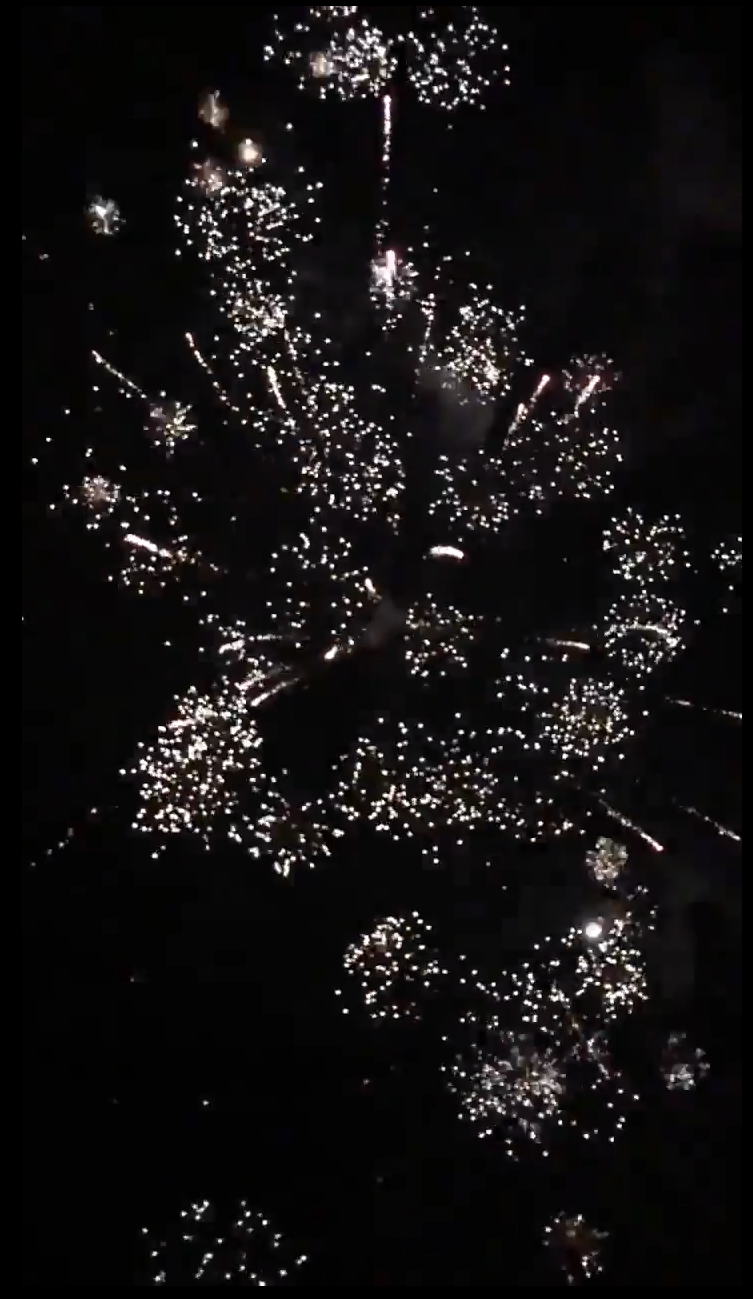
\includegraphics[width=0.35\textwidth]{fireworks.png}

\small\textit{Original fireworks image}
\end{center}

\end{stepbox}

\begin{stepbox}[Step 2: Evaluate Available Operations]

We can categorize image processing operations by their effect:

\vspace{0.3cm}
\textbf{Category A: Operations that brighten dark regions}

These operations attempt to reveal detail in shadows by lifting dark intensities.

\begin{center}
\begin{tabular}{ccc}
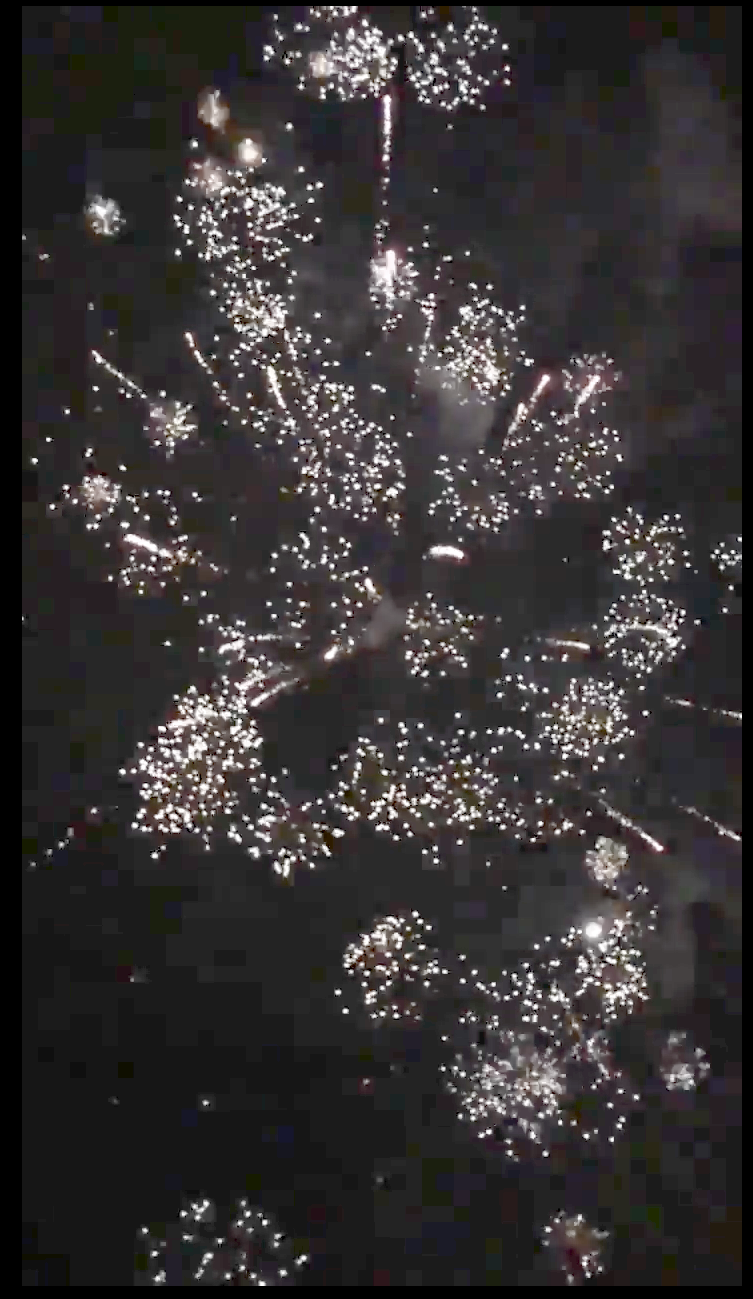
\includegraphics[width=0.28\textwidth]{fireworks_gamma.png} &
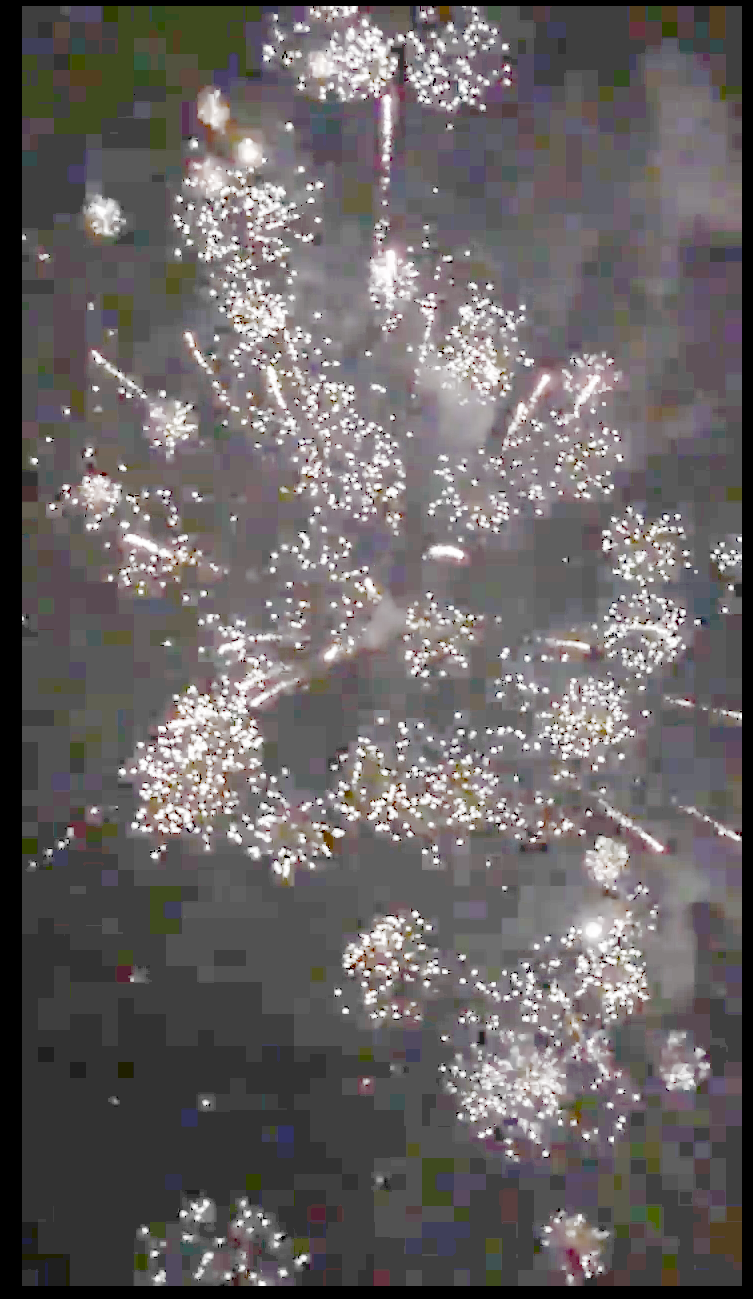
\includegraphics[width=0.28\textwidth]{fireworks_log.png} &
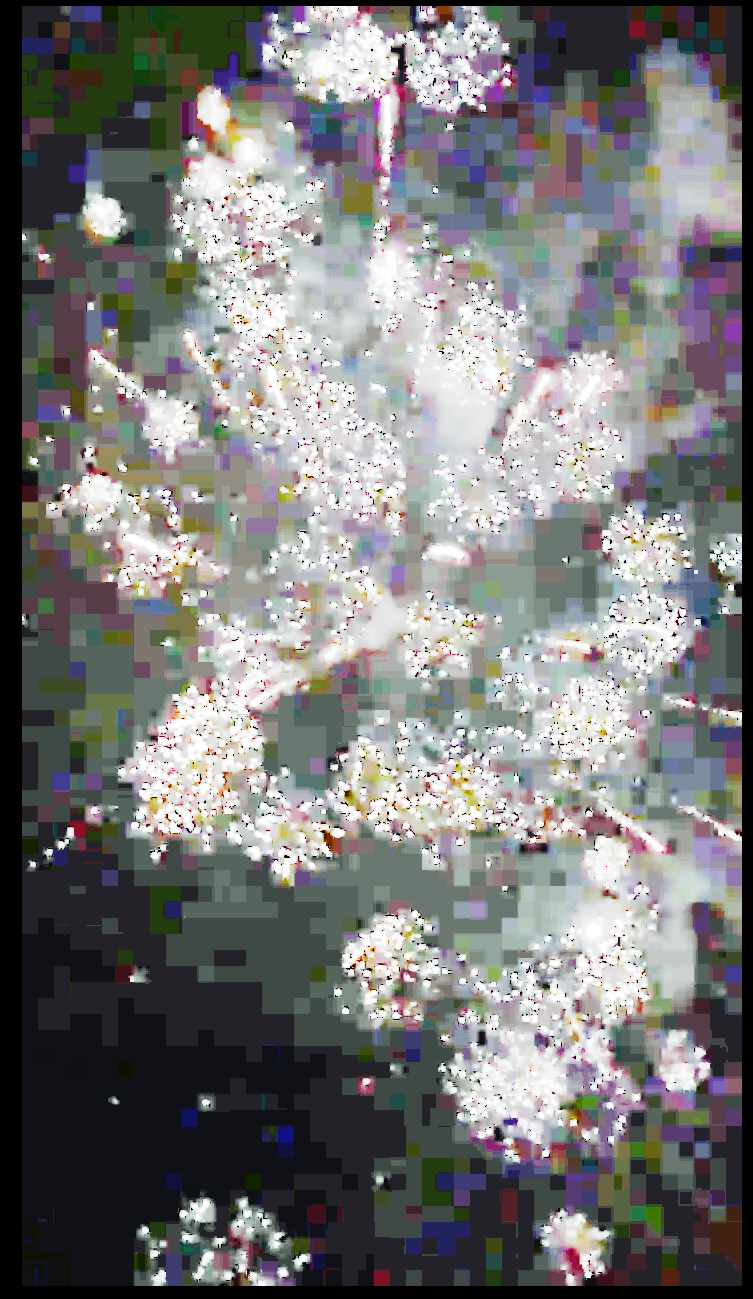
\includegraphics[width=0.28\textwidth]{fireworks_histeq.png} \\
\small Gamma ($\gamma = 0.5$) & \small Log Transform & \small Histogram Equalization
\end{tabular}
\end{center}

\textbf{Effect}: The black sky becomes gray, revealing noise and sensor artifacts. This is \textbf{undesirable} for fireworks because the sky \textit{should} be black---there is no meaningful information to reveal.

\vspace{0.3cm}
\textbf{Category B: Operations that increase contrast (darks darker, lights lighter)}

These operations push dark values toward black and light values toward white.

\begin{center}
\begin{tabular}{cc}
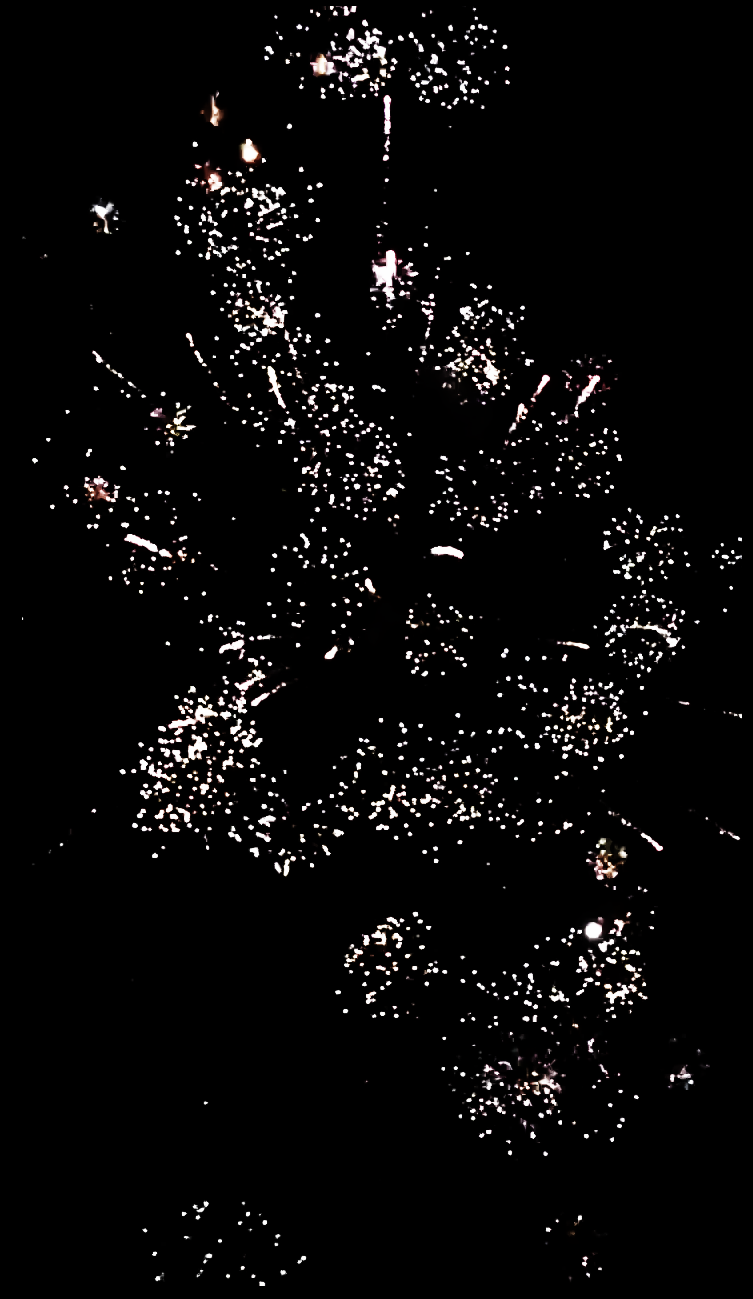
\includegraphics[width=0.35\textwidth]{fireworks_scurve.png} &
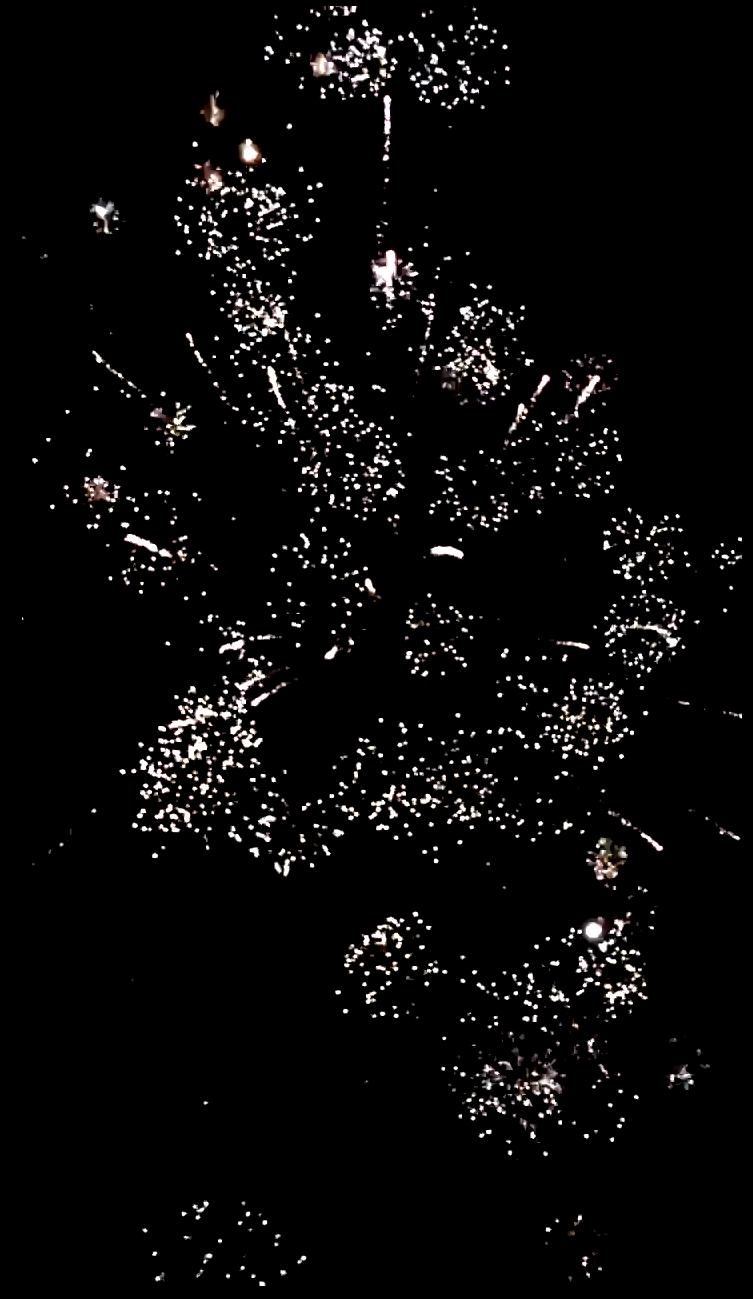
\includegraphics[width=0.35\textwidth]{fireworks_boosted.png} \\
\small S-Curve Contrast & \small Boosted Contrast
\end{tabular}
\end{center}

\textbf{Effect}: The sky becomes pure black while the fireworks remain bright. This is \textbf{desirable} for aesthetic night photography.

\vspace{0.3cm}
\textbf{Category C: Sharpening operations}

These operations enhance edges and fine details.

\begin{center}
\begin{tabular}{cc}
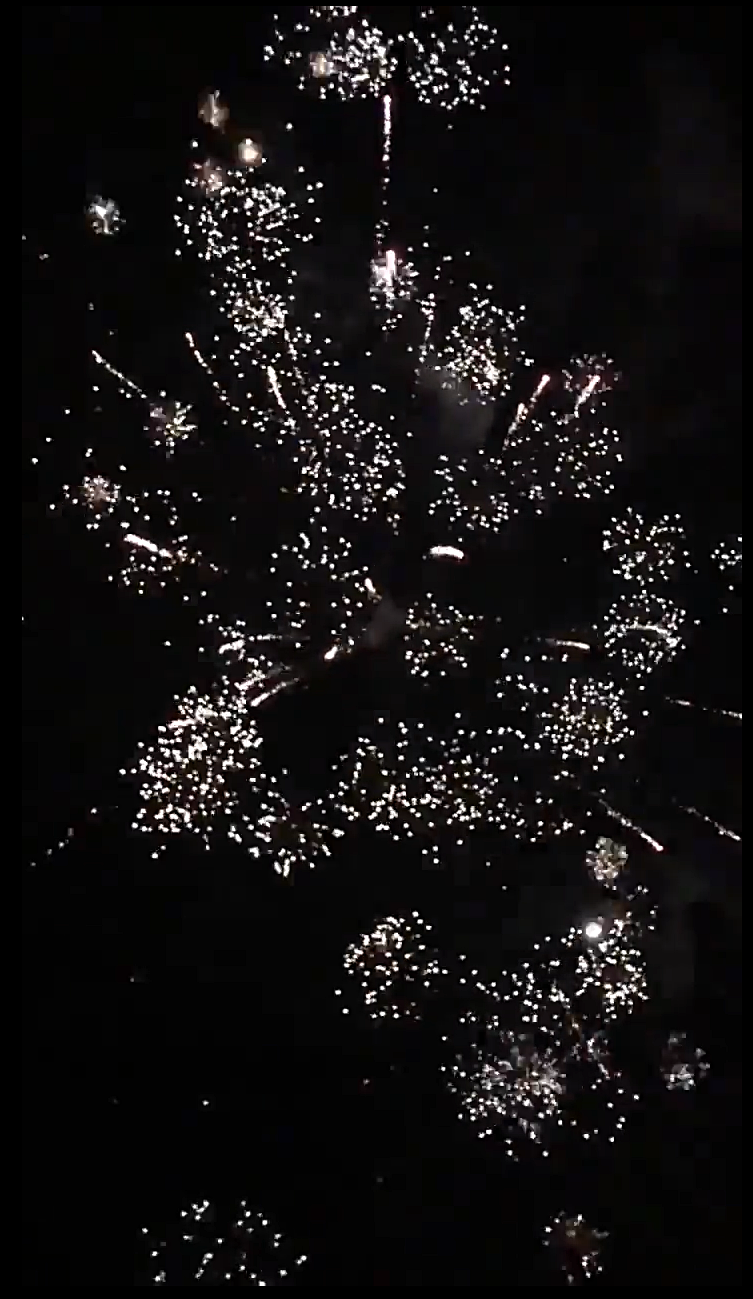
\includegraphics[width=0.35\textwidth]{fireworks_sharpened.png} &
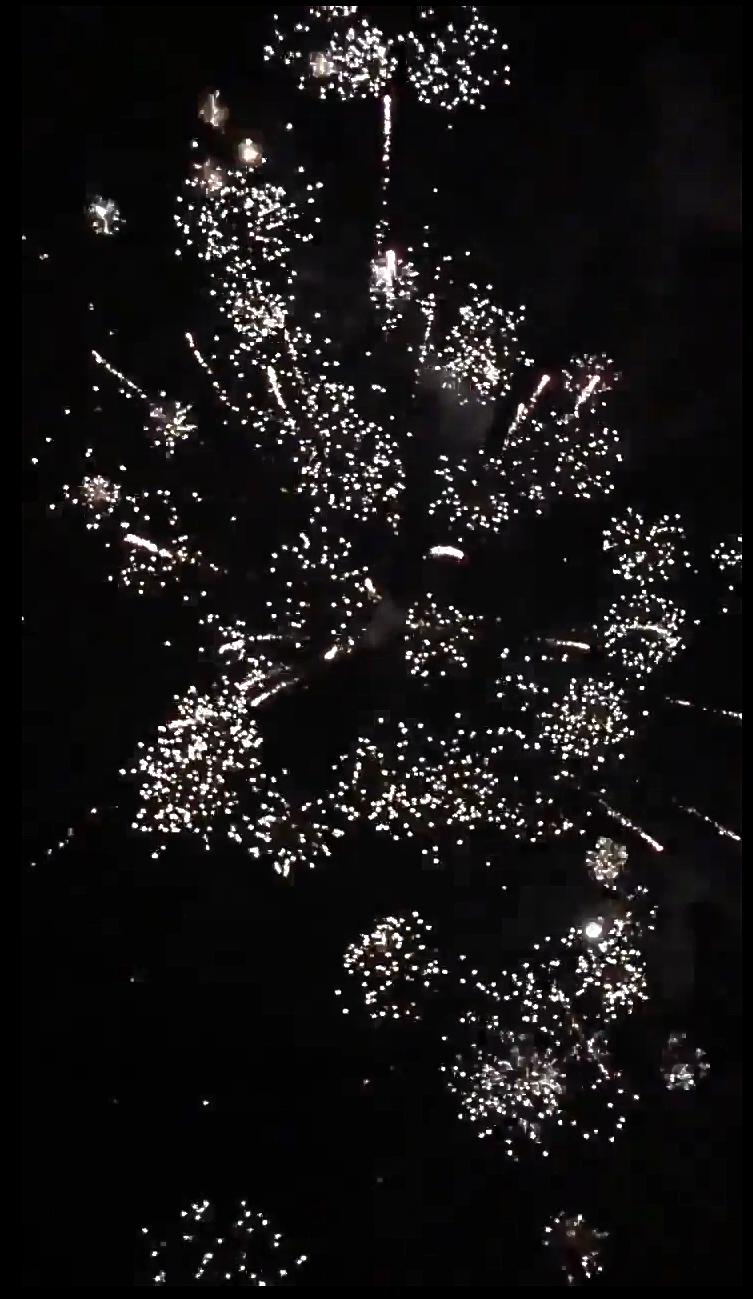
\includegraphics[width=0.35\textwidth]{fireworks_highboost.png} \\
\small Unsharp Masking & \small High-Boost Filtering
\end{tabular}
\end{center}

\textbf{Effect}: Firework sparks appear crisper with more defined edges.

\vspace{0.3cm}
\textbf{Category D: Color enhancement}

\begin{center}
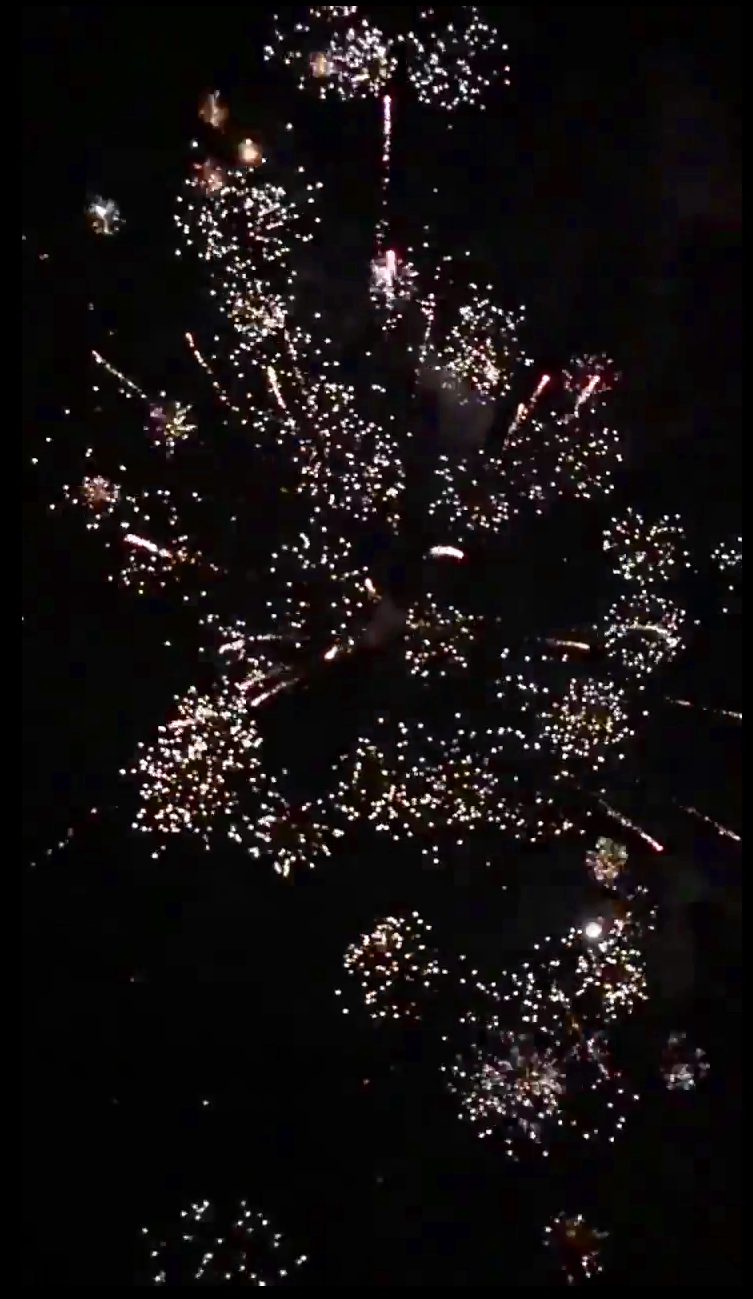
\includegraphics[width=0.35\textwidth]{fireworks_saturated.png}

\small Saturation Boost
\end{center}

\textbf{Effect}: Colors become more vivid and vibrant.

\end{stepbox}

\begin{stepbox}[Step 3: Consider the Optimization Goal]

The ``correct'' operations depend entirely on what you are trying to achieve:

\vspace{0.2cm}
\begin{center}
\begin{tabular}{|l|l|l|}
\hline
\textbf{Goal} & \textbf{Recommended Operations} & \textbf{Avoid} \\
\hline
Aesthetic (fireworks) & S-curve, sharpening, saturation & Gamma, Hist EQ \\
\hline
Surveillance (reveal shadows) & Gamma, log transform, Hist EQ & S-curve \\
\hline
Medical imaging & CLAHE, careful contrast & Extreme transforms \\
\hline
Object detection & Thresholding, edge detection & Aesthetic enhancements \\
\hline
\end{tabular}
\end{center}

\vspace{0.2cm}

The same operation can be \textit{beneficial} or \textit{harmful} depending on the goal. Histogram equalization is excellent for revealing hidden details in surveillance footage, but terrible for fireworks photography where the dark background should remain dark.

\end{stepbox}

\begin{stepbox}[Step 4: Consider the Display Medium]

The target display device also affects which operations are most beneficial:

\vspace{0.2cm}
\begin{center}
\begin{tabular}{|l|l|l|}
\hline
\textbf{Display} & \textbf{Prioritize} & \textbf{Less Important} \\
\hline
Mobile phone (small screen) & Color, contrast, brightness & Fine sharpening \\
\hline
Desktop monitor (large screen) & Sharpness, fine detail & Can be subtle \\
\hline
Print & Resolution, color accuracy & Different gamma curve \\
\hline
\end{tabular}
\end{center}

\vspace{0.2cm}

On a mobile phone, viewers cannot resolve fine detail, so aggressive sharpening provides little benefit---but punchy colors and contrast help images ``pop'' on a small screen viewed in variable lighting. On a desktop monitor, fine details are visible, making sharpening more valuable.

\end{stepbox}

\begin{resultsbox}

\textbf{Recommended operations for fireworks photography:}

\begin{enumerate}[leftmargin=2em]
\item \textbf{S-curve contrast enhancement}: Apply a sigmoid transformation $s = \frac{1}{1 + e^{-k(r-0.5)}}$ to push dark pixels darker and bright pixels brighter. This ensures a pure black sky while maintaining bright firework sparks.

\item \textbf{Saturation boost} (especially for mobile display): Increase color saturation to make the firework colors more vivid and visually striking.

\item \textbf{Sharpening} (especially for desktop/print): Apply unsharp masking or high-boost filtering to enhance the crispness of firework spark edges.
\end{enumerate}

\vspace{0.2cm}
\textbf{Operations to avoid}: Gamma correction ($\gamma < 1$), log transforms, and histogram equalization---these lift the dark sky and reveal noise, degrading the aesthetic quality.

\end{resultsbox}

\newpage

% ============================================================================
% PROBLEM 2
% ============================================================================

\problem{Problem 2) (20 points)}

A, B, C and D are four sets. Give expressions for the set shown shaded in Figure 2 in terms of A,
B, C, and D. Note that all of the shaded areas constitute of one set

% --- Individual shapes A, B, C, D ---
\begin{center}
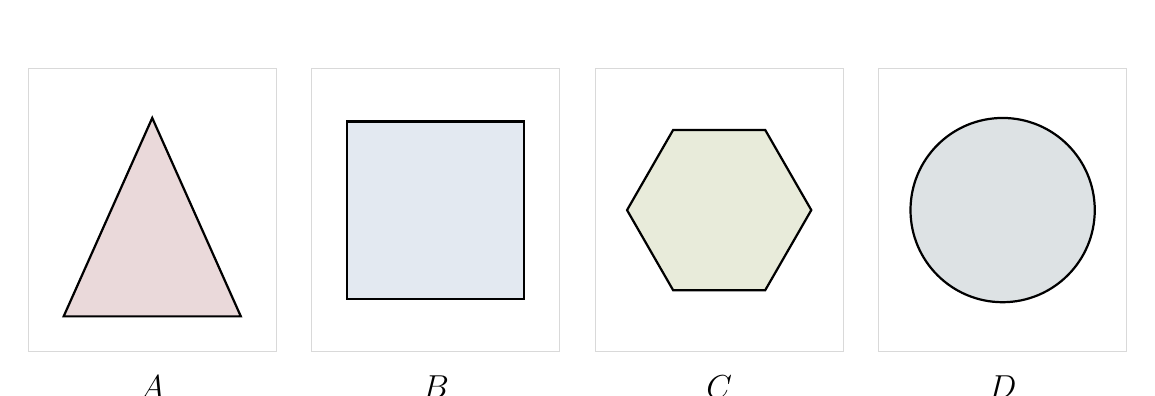
\begin{tikzpicture}[scale=0.9]

    % === Shape A (Triangle) - centered and filling box ===
    \begin{scope}[shift={(0,0)}]
        \draw[gray!30, thin] (-0.5,-0.5) rectangle (3,3.5);
        \fill[USC_Garnet!15] (0,0) -- (2.5,0) -- (1.25,2.8) -- cycle;
        \draw[thick] (0,0) -- (2.5,0) -- (1.25,2.8) -- cycle;
        \node[font=\large\bfseries] at (1.25, -1) {$A$};
    \end{scope}

    % === Shape B (Rectangle) - centered and filling box ===
    \begin{scope}[shift={(4,0)}]
        \draw[gray!30, thin] (-0.5,-0.5) rectangle (3,3.5);
        \fill[USC_Atlantic!15] (0,0.25) rectangle (2.5,2.75);
        \draw[thick] (0,0.25) rectangle (2.5,2.75);
        \node[font=\large\bfseries] at (1.25, -1) {$B$};
    \end{scope}

    % === Shape C (Hexagon) - centered and filling box ===
    \begin{scope}[shift={(8,0)}]
        \draw[gray!30, thin] (-0.5,-0.5) rectangle (3,3.5);
        % Hexagon centered at (1.25, 1.5) with radius 1.3
        \fill[USC_Honeycomb!15] (2.55,1.5) -- (1.9,2.63) -- (0.6,2.63) -- (-0.05,1.5) -- (0.6,0.37) -- (1.9,0.37) -- cycle;
        \draw[thick] (2.55,1.5) -- (1.9,2.63) -- (0.6,2.63) -- (-0.05,1.5) -- (0.6,0.37) -- (1.9,0.37) -- cycle;
        \node[font=\large\bfseries] at (1.25, -1) {$C$};
    \end{scope}

    % === Shape D (Circle) - centered and filling box ===
    \begin{scope}[shift={(12,0)}]
        \draw[gray!30, thin] (-0.5,-0.5) rectangle (3,3.5);
        \fill[USC_Congaree!15] (1.25,1.5) circle (1.3);
        \draw[thick] (1.25,1.5) circle (1.3);
        \node[font=\large\bfseries] at (1.25, -1) {$D$};
    \end{scope}

\end{tikzpicture}
\end{center}

\vspace{0.3cm}

% Path macros for shape definitions (in combined diagram coordinates)
\newcommand{\pathA}{(0.297,1.237) -- (1.857,1.237) -- (1.077,2.919) -- cycle}
\newcommand{\pathB}{(1.501,0.798) rectangle (2.887,2.184)}
\newcommand{\pathD}{(1.458,0.863) circle (0.881)}
\newcommand{\pathC}{(2.616,0.805) -- (2.220,1.492) -- (1.426,1.492) -- (1.030,0.805) -- (1.426,0.118) -- (2.220,0.118) -- cycle}

% --- Combined diagram with shaded regions ---
\begin{center}
\begin{tikzpicture}[scale=2.2]

    % ============================
    % Shaded region 1: (A ∩ D) - B - C
    % ============================
    % First fill A ∩ D
    \begin{scope}
        \clip \pathA;
        \clip \pathD;
        \fill[pattern=north east lines] (-1,-1) rectangle (5,4);
    \end{scope}
    % Remove A ∩ D ∩ B
    \begin{scope}
        \clip \pathA;
        \clip \pathD;
        \clip \pathB;
        \fill[white] (-1,-1) rectangle (5,4);
    \end{scope}
    % Remove A ∩ D ∩ C
    \begin{scope}
        \clip \pathA;
        \clip \pathD;
        \clip \pathC;
        \fill[white] (-1,-1) rectangle (5,4);
    \end{scope}

    % ============================
    % Shaded region 2: (D ∩ B) - A - C
    % ============================
    % First fill D ∩ B
    \begin{scope}
        \clip \pathD;
        \clip \pathB;
        \fill[pattern=north east lines] (-1,-1) rectangle (5,4);
    \end{scope}
    % Remove D ∩ B ∩ A
    \begin{scope}
        \clip \pathD;
        \clip \pathB;
        \clip \pathA;
        \fill[white] (-1,-1) rectangle (5,4);
    \end{scope}
    % Remove D ∩ B ∩ C
    \begin{scope}
        \clip \pathD;
        \clip \pathB;
        \clip \pathC;
        \fill[white] (-1,-1) rectangle (5,4);
    \end{scope}

    % ============================
    % Shaded region 3: (B ∩ C) - A - D
    % ============================
    % First fill B ∩ C
    \begin{scope}
        \clip \pathB;
        \clip \pathC;
        \fill[pattern=north east lines] (-1,-1) rectangle (5,4);
    \end{scope}
    % Remove B ∩ C ∩ A
    \begin{scope}
        \clip \pathB;
        \clip \pathC;
        \clip \pathA;
        \fill[white] (-1,-1) rectangle (5,4);
    \end{scope}
    % Remove B ∩ C ∩ D
    \begin{scope}
        \clip \pathB;
        \clip \pathC;
        \clip \pathD;
        \fill[white] (-1,-1) rectangle (5,4);
    \end{scope}

    % Draw all shape outlines (no labels)
    \draw[thick] \pathA;
    \draw[thick] \pathB;
    \draw[thick] \pathD;
    \draw[thick] \pathC;

\end{tikzpicture}
\end{center}

\newpage

% ============================================================================
% PROBLEM 3
% ============================================================================

\problem{Problem 3) (25 points)}

Given a 3x3 spatial filter $\displaystyle\frac{1}{9}\begin{bmatrix} -1 & -1 & -1 \\ -1 & -17 & -1 \\ -1 & -1 & -1 \end{bmatrix}$ answer the following questions:

\begin{enumerate}
\item (10 points) What type of filter is it? When applying this filter on an image, what kind of effect you
will expect in the output image? Why? (Hint: is this filter an image smoothing filter, an
image sharpening filter or an edge detector?)

\item (15 points) Perform the image convolution using this filter on a 3x3 image $\begin{bmatrix} 3 & 5 & 12 \\ 7 & 18 & 11 \\ 5 & 9 & 15 \end{bmatrix}$. Give the
CROPPED filtering result for the output image. (Hint: you need to assume an appropriate
zero mapping)
\end{enumerate}

\newpage

% ============================================================================
% PROBLEM 4
% ============================================================================

\problem{Problem 4) (25 points)}

An image with intensities in the range $r \in [0, L-1]$ has the pdf

\[
p_r(r) = \begin{cases} \displaystyle\frac{4r}{3(L-1)^2} & 0 \le r \le L-1 \\[0.5em] 0 & \text{otherwise} \end{cases}
\]

where $L-1$ is the maximum intensity value. It is desired to transform the intensity levels of this image so that they will have the specified pdf

\[
p_z(z) = \begin{cases} \displaystyle\frac{2z}{(L-1)^2} & 0 \le z \le L-1 \\[0.5em] 0 & \text{otherwise} \end{cases}
\]

Assume that the intensity value is continuous and find the transformation function $z = T(r)$ in terms of $r$ and $z$ that will accomplish this.

\vspace{0.5cm}

(Hints: The transformation function of histogram equalization is given as

\[
s = T(r) = (L-1) \int_0^r p_r(w)\,dw
\]
)

\newpage

% ============================================================================
% BONUS QUESTION
% ============================================================================

\begin{center}
\textbf{Bonus Question (20 points)}
\end{center}

Perform the Fourier transform to a function as shown in Figure 3.

\vspace{0.3cm}

(Hint: the definition of the Fourier transform of a function is $\displaystyle F(u) = \int_{-\infty}^{\infty} f(t) e^{-j2\pi ut}\,dt$ )

\begin{center}
\begin{tikzpicture}[scale=0.85]
    % Axes
    \draw[->] (-4,0) -- (5,0) node[right] {$t$};
    \draw[->] (0,-0.5) -- (0,4) node[above] {$f(t)$};

    % Tick marks on x-axis
    \foreach \x in {-3,-2,-1,1,2,3,4} {
        \draw (\x,0.08) -- (\x,-0.08) node[below] {\small $\x$};
    }
    \node[below] at (0,-0.08) {\small $0$};

    % Tick marks on y-axis
    \foreach \y in {1,2,3} {
        \draw (0.08,\y) -- (-0.08,\y) node[left] {\small $\y$};
    }

    % The step function: 3 from -2 to -1, 2 from -1 to 2, 3 from 2 to 4
    \draw[thick] (-3.5,0) -- (-2,0);         % zero before -2
    \draw[thick] (-2,0) -- (-2,3);           % rise to 3 at -2
    \draw[thick] (-2,3) -- (-1,3);           % plateau at 3
    \draw[thick] (-1,3) -- (-1,2);           % drop to 2 at -1
    \draw[thick] (-1,2) -- (2,2);            % plateau at 2 (middle)
    \draw[thick] (2,2) -- (2,3);             % rise to 3 at 2
    \draw[thick] (2,3) -- (4,3);             % plateau at 3
    \draw[thick] (4,3) -- (4,0);             % drop to 0 at 4
    \draw[thick] (4,0) -- (4.5,0);           % zero after 4
\end{tikzpicture}
\end{center}

% ============================================================================
% END OF DOCUMENT
% ============================================================================

\end{document}
